\documentclass{article}
\usepackage{color}
\usepackage{soul}
\usepackage{multirow}
\usepackage{pgfplots}
\usepackage{ifthen}
\usepackage[UTF8]{ctex}
\usepackage[left=3.0cm,right=3.0cm,top=2.5cm,bottom=2.5cm]{geometry}
\geometry{a4paper}
\usepackage{tikz}
\usetikzlibrary{chains}
\newcommand{\diff}{\mathop{}\!\mathrm{d}}
\usepackage{appendix} 
\usepackage{lipsum}
\usepackage{listings}
\usepackage{diagbox}
\usepackage{pdfpages}
\usepackage{xcolor}
\usepackage{pdflscape}
\usepackage{soul}
\usepackage{booktabs}
\usepackage{longtable}
\usepackage[most]{tcolorbox}
\newtcolorbox{mycolorbox}[1][]{
  sharp corners,
  colback=white, 
  colframe=black, 
  coltext=blue, 
  boxsep=5pt, 
  left=2pt, 
  right=2pt, 
  top=1pt, 
  bottom=1pt,
  breakable,
  #1 
}
\usepackage{subcaption}
\lstset{
    backgroundcolor=\color{gray!20},
    basicstyle=\ttfamily,
    commentstyle=\color{darkgray}\ttfamily,
    stringstyle=\color{red},
    showstringspaces=false,
    numbers=left,
    numberstyle=\tiny\color{gray},
    stepnumber=1,
    numbersep=10pt,
    tabsize=4,
    showspaces=false,
    showtabs=false,
    frame=single,
    captionpos=b,
    breaklines=true,
    breakatwhitespace=false,
    escapeinside={\%*}{*)},
    xleftmargin=\parindent,
    xrightmargin=\parindent,
}
\lstdefinestyle{dockerstyle}{
    language=bash,
    keywordstyle=\color{blue}\bfseries,
    morekeywords={FROM, RUN, CMD, LABEL, EXPOSE, ENV, ADD, COPY, ENTRYPOINT, VOLUME, USER, WORKDIR, ARG, ONBUILD},
}
\lstdefinestyle{pythonstyle}{
    language=Python,
    keywordstyle=\color{blue}\bfseries,
    morekeywords={import, from, as, def, return, class, self, if, elif, else, while, for, try, except, with},
}
\lstdefinestyle{cstyle}{
    language=C,
    keywordstyle=\color{blue}\bfseries,
    morekeywords={size_t, printf}, 
}
\lstdefinestyle{bashstyle}{
    language=bash,
    keywordstyle=\color{blue}\bfseries,
    morekeywords={echo,sudo ,if, then, else, fi, for, in, do, done, echo, exit, return, function},
    commentstyle=\color{green}\ttfamily,
}
\usepackage{algorithm}
\usepackage{algpseudocode}
\renewcommand{\algorithmicrequire}{\textbf{Input:}}  
\renewcommand{\algorithmicensure}{\textbf{Output:}}  
\usepackage{amsmath}
\usepackage{amsthm}
\DeclareMathOperator{\sigm}{sigm}
\usepackage{graphicx}
\usepackage{float}
\renewcommand{\vec}[1]{\boldsymbol{#1}}
\usepackage{amssymb}
\usepackage{booktabs} 
\usepackage{hyperref}
\usepackage{titlesec}
\usepackage{caption}
\usepackage{fontspec}
\usepackage{xeCJK}
\setCJKmainfont{SimSun} 
\title{\Huge 数据库(2)实验2}
\author{21121178 王士博}
\begin{document}
\begin{center}
    \textbf{\huge 数据库(2)实验1:云服务器部署Mysql}
\end{center}
\begin{center}
    \textbf{\large \textbf{学号:21121178 \quad 姓名:王士博 \quad 指导教师:刘洋}}
\end{center}
\hrulefill
\section{实验环境}
\begin{itemize}
    \item 腾讯云服务器配置:竞价实例,香港地区,标准型SA5,8核 16GB,Ubuntu 20.04。
\end{itemize}
\section{实验目的}
\section{实验步骤}
\subsection{创建一个包含docker和kubernetes的镜像}
先购买一个实例,然后通过如下的命令安装docker,这下面的指令包括了三部分:
\begin{enumerate}
    \item 安装三个证书工具:\texttt{ca-certificates},\texttt{curl},\texttt{gnupg},这些证书
    工具用于下载所需要的证书,处理所需要的证书和使用一些加密技术。
    \item 下载Docker的GPG公钥:使用Docker的公钥对下载的安装包进行验证,/etc/apt/keyrings/
    目录转门放置apt下载包的公钥环,用于验证安装包。
    \item 下载Docker,并且执行Docker hello-world测试Docker的拉取镜像和创建实例的能力是否正确依次来验证
    Docker是否安装成功。
\end{enumerate}
其中下载Docker包括下面几个步骤,更新应用商店确保下载的所有内容都是最新的,使用下载的证书工具下载Docker的GPG公钥,
最后下载Docker的指定版本并且运行hello-world测试,下面省略部分指令,只保留
制定版本号的指令以便复现,剩余的指令可以在\url{https://docs.docker.com/engine/install/ubuntu/}
找到,安装结果如图\ref{fig:dockerinstall},
测试结果如图\ref{fig:helloworld}所示。
\begin{lstlisting}[style=bashstyle]
apt list -a docker-ce
sudo apt-get install docker-ce=5:19.03.10~3-0~ubuntu-focal
sudo docker run hello-world
\end{lstlisting}
下面先更换下载kubernetes的源为Aliyun的源,然后安装kubernetes,安装kubernetes的指令如下,结果如图\ref{fig:kubernetesverification}所示
(\textcolor{red}{注}:这里的kubernetes必须安装制定的版本,过高版本会产生和Docker的适配问题)。
\begin{lstlisting}[style=bashstyle]
sudo apt-get install apt-transport-https
curl https://mirrors.aliyun.com/kubernetes/apt/doc/apt-key.gpg | sudo apt-key add - 
sudo vim /etc/apt/sources.list.d/kubernetes.list
sudo apt-get update
apt-cache madison kubeadm
sudo apt-get install -y kubelet=1.18.0-00 kubeadm=1.18.0-00 kubectl=1.18.0-00
kubeadm version
\end{lstlisting}
实验结果如图所示: \\
\noindent
\begin{minipage}{0.45\textwidth}
    \begin{figure}[H]
        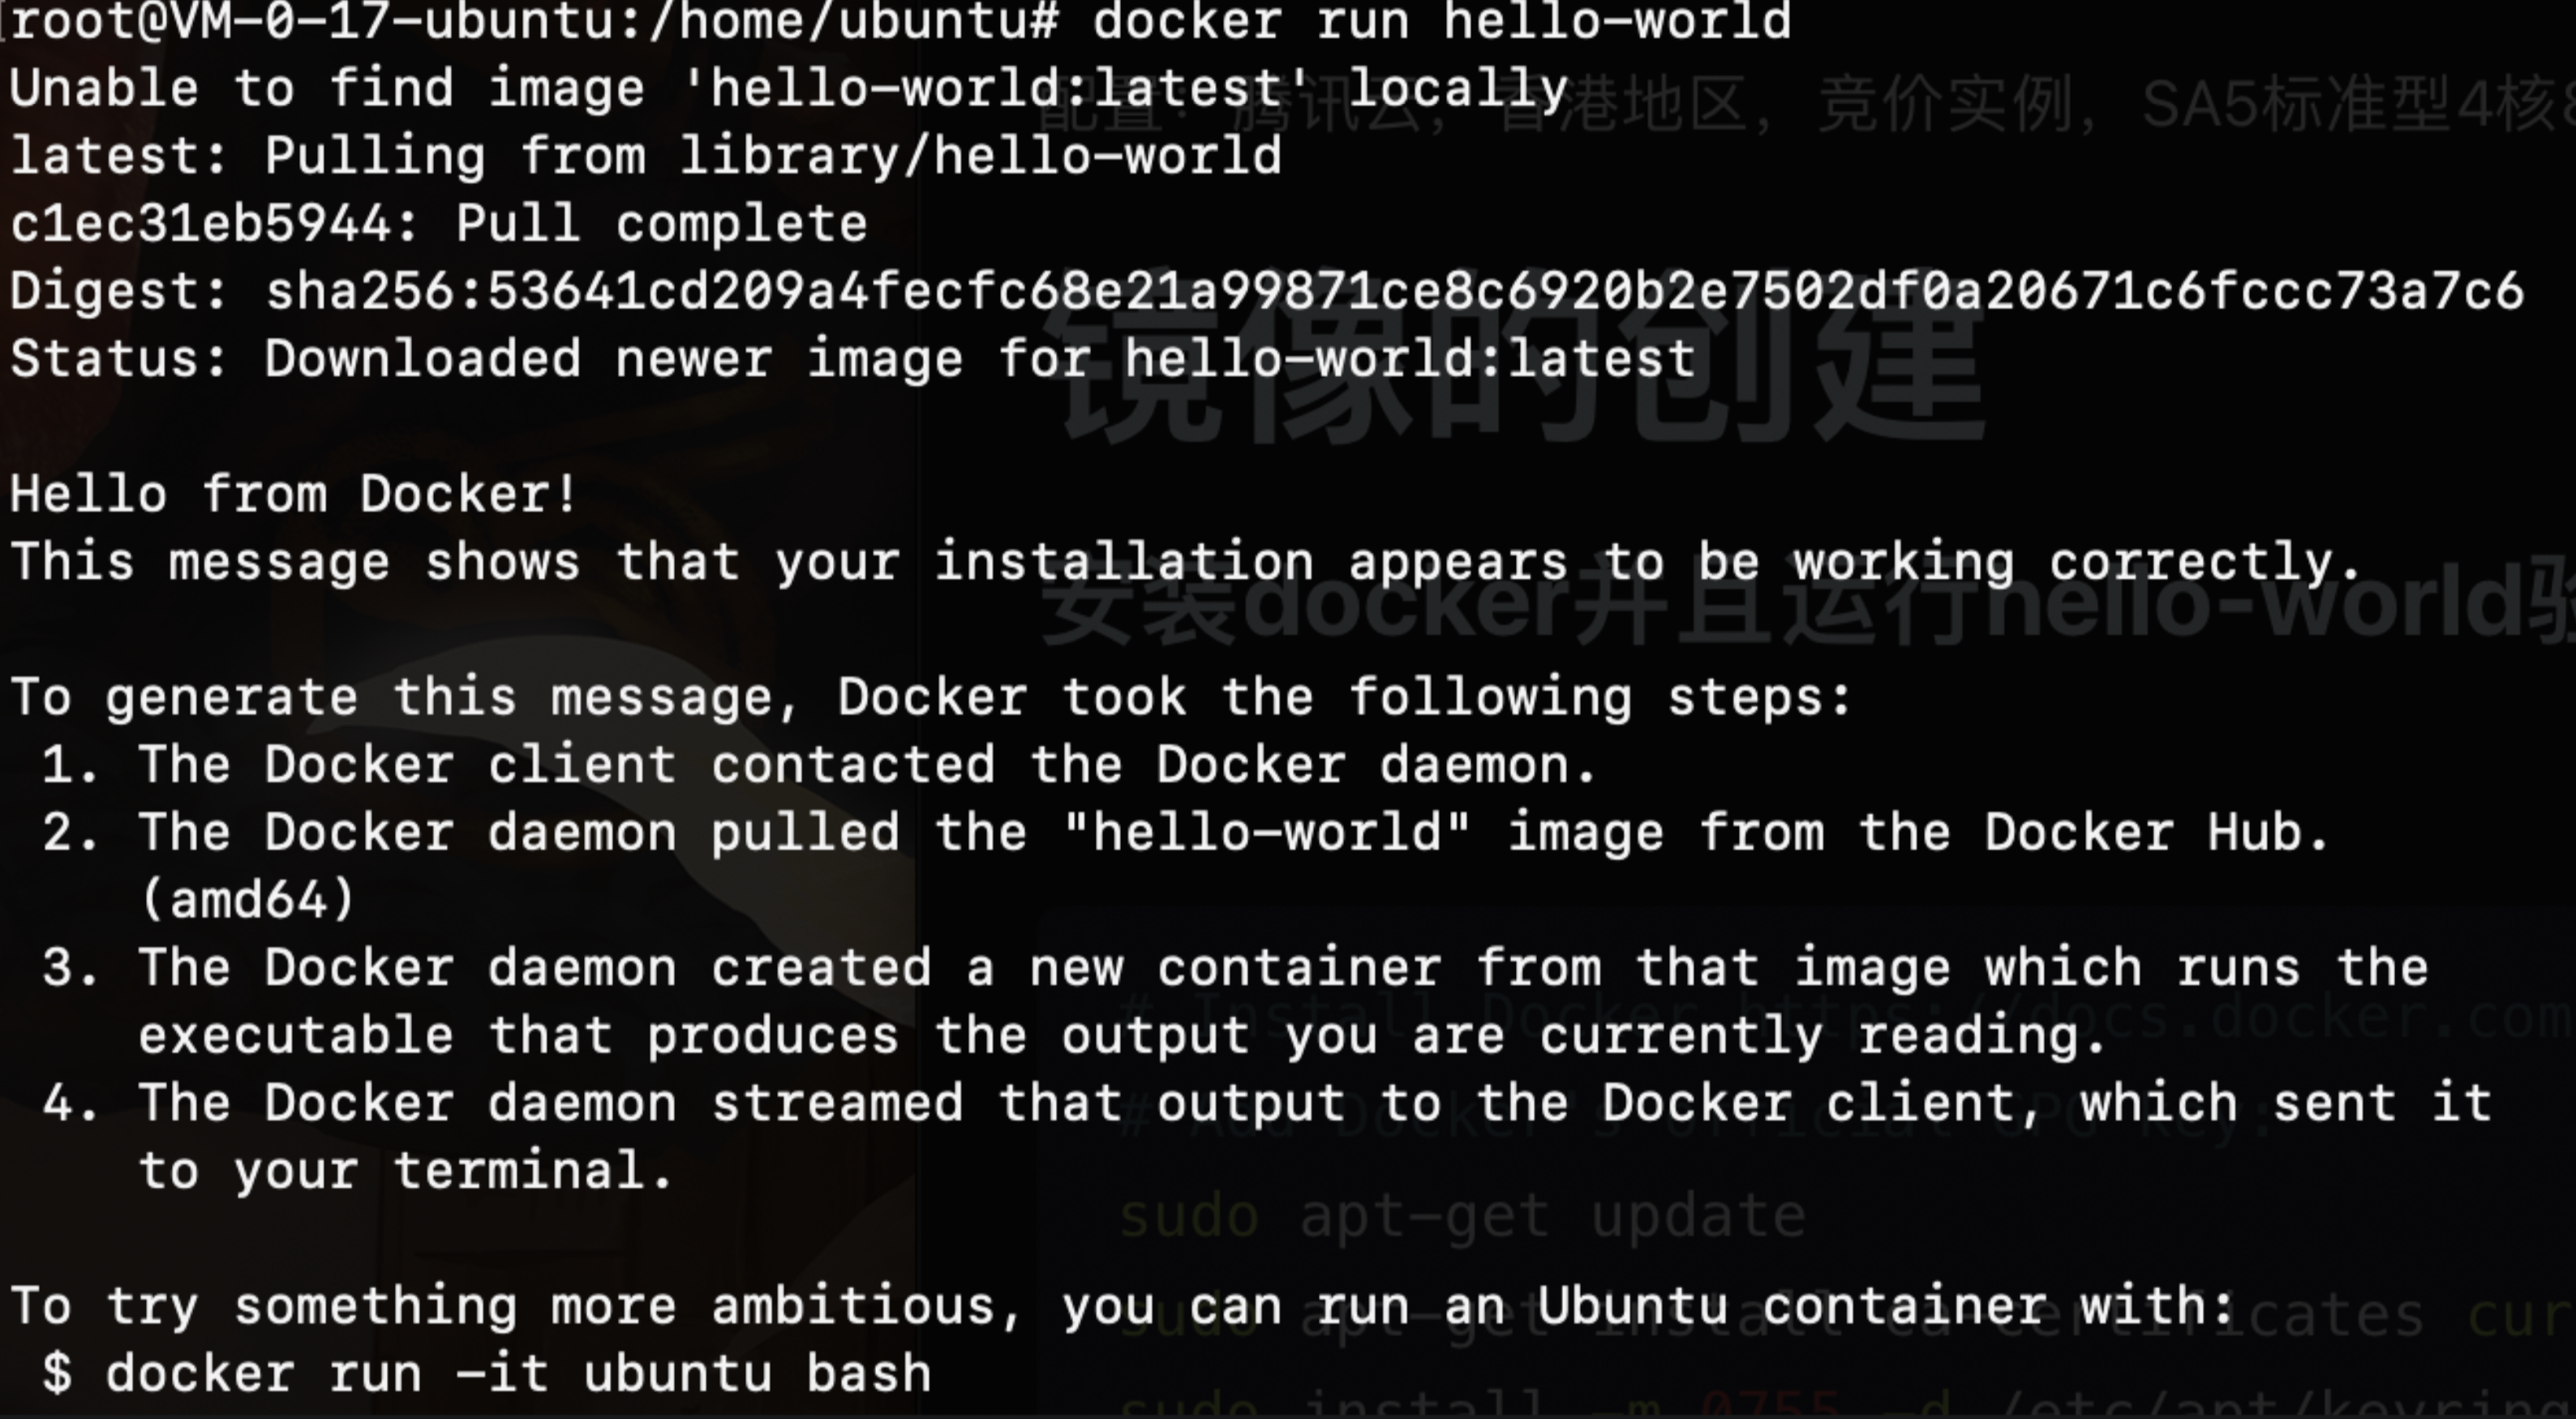
\includegraphics[width=\textwidth]{dockerhelloworld.png}
        \caption{docker安装}
        \label{fig:dockerinstall}
    \end{figure}
\end{minipage}
\hfill
\begin{minipage}{0.45\textwidth}
    \begin{figure}[H]
        \centering
        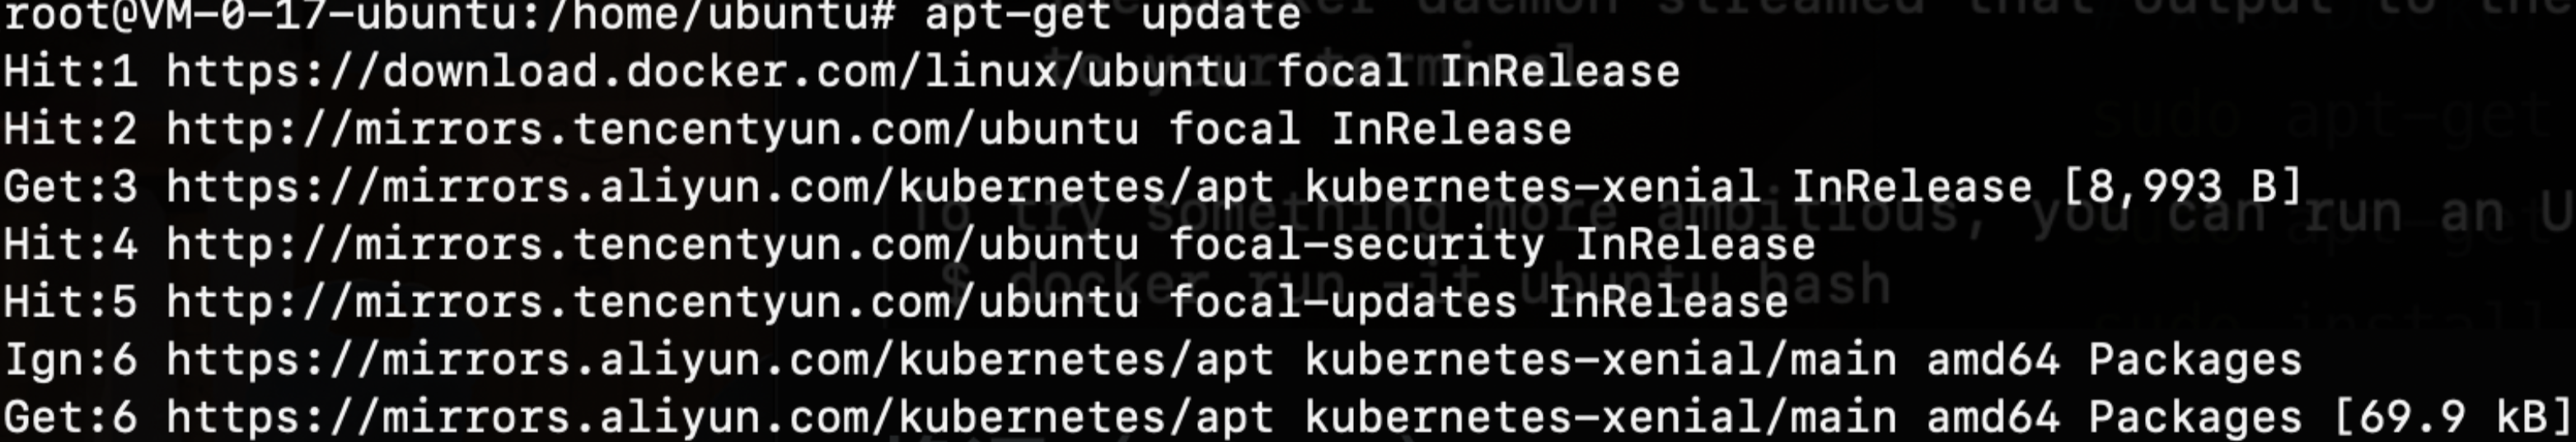
\includegraphics[width=1.0\textwidth]{changeorigin.png}
        \caption{docker hello-world}
        \label{fig:helloworld}
    \end{figure}
    \begin{figure}[H]
        \centering
        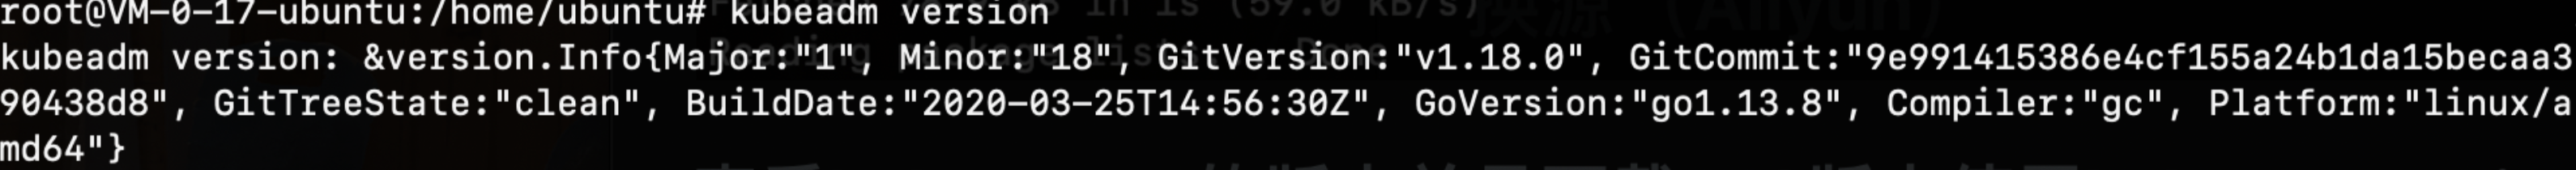
\includegraphics[width=1.0\textwidth]{kubernetesverify.png}
        \caption{kubernetes-verification}
        \label{fig:kubernetesverification}
    \end{figure}
\end{minipage}

\subsection{创建kubernetes集群}
\indent 通过上面导出的镜像来创建下面三个实例,通过修
改\texttt{/etc/hostname}和\texttt{/etc/hosts}文件改变三台主机的主机名
以及配置IP地址和hostname的映射。
然后在Boss实例上开启kubernetes集群,然后在fw1和fw2上加入集群。,使用如下指令开启kubernetes集群,
这其中指定了API Server的内网地址,这是让其他节点可以访问到kubernetes的API地址,也就是master节点的地址,
kubernetes的网络配置有三层,节点通信网络,服务通信子网,实例通信子网,节点之间通过他们的互联网络(子网IP,公网IP)进行通讯
,实例之间通过实例子网进行通讯,服务通过将很多个相同作用的实例进行封装成统一的端口进行访问。然后fw1和fw2作为Worker节点
使用下面的命令加入集群,这条指令包括了加入集群的token和ca证书的hash值,这个hash值是用来验证token的合法性的。
\begin{lstlisting}[style=bashstyle]
# 在Boss实例上执行
sudo kubeadm init --apiserver-advertise-address=172.19.0.14 --image-repository registry.aliyuncs.com/google_containers --service-cidr=10.96.0.0/12  --pod-network-cidr=10.244.0.0/16
# 在fw1和fw2上执行
kubeadm join 172.19.0.14:6443 --token gc92e7.mhcy04py9yamyu04 \
    --discovery-token-ca-cert-hash sha256:4fef2226583d439cdce103242769c4ecc860a6733556a0e39c31f9d202620d5c
\end{lstlisting}
通过加入集群,master节点可以根据网络带宽资源等条件将一些容器或者服务分配到workder节点上维护或者运行
实现负载均衡,首先通过执行如下的指令配置kubectl,这两条指令将root用户的配置文件复制到普通用户
的目录下,然后更改文件的权限以此达到普通用户也可以使用kubectl的目的。
\begin{lstlisting}[style=bashstyle]
mkdir -p $HOME/.kube
sudo cp -i /etc/kubernetes/admin.conf $HOME/.kube/config
sudo chown $(id -u):$(id -g) $HOME/.kube/config
\end{lstlisting}
然后使用\texttt{kubectl apply -f \$\{url\} }来应用flannel的网络配置方案。可以通过\texttt{kubectl get nodes}
来查看加入集群的节点,通过\texttt{kubectl get pods}查看当前运行的实例,通过\texttt{kubectl get services}查看当
前运行的服务。
\begin{figure}[H]
    \begin{subfigure}[b]{0.3\textwidth}
        \centering
        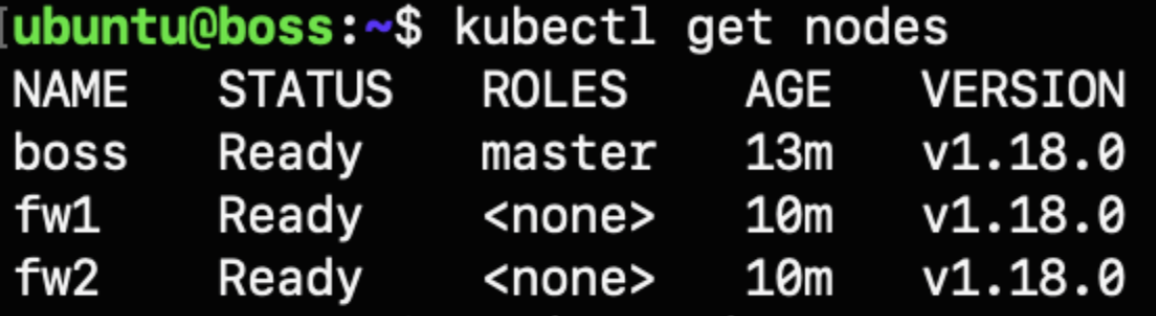
\includegraphics[width=\textwidth]{nodes.png}
        \caption{获取加入节点的数量和信息}
        \label{fig:nodes1}
    \end{subfigure}
    \hfill
    \begin{subfigure}[b]{0.65\textwidth}
        \centering
        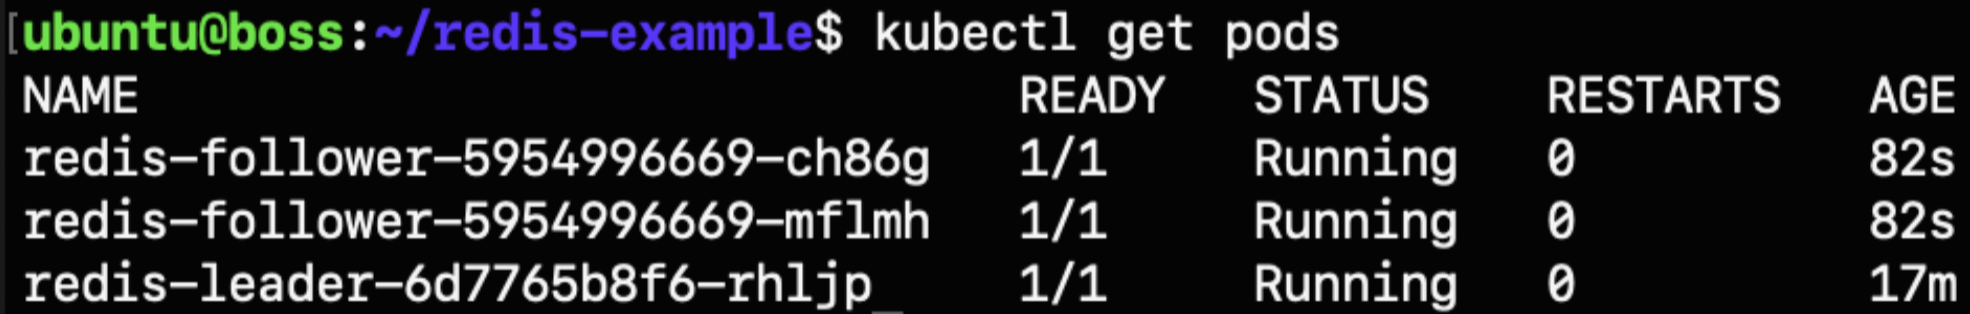
\includegraphics[width=\textwidth]{pods.png}
        \caption{获取当前运行的实例}
        \label{fig:pods1}
    \end{subfigure}
\end{figure}
\subsection{验证Kubernetes的特性}
\begin{enumerate}
    \item {\textbf{\heiti 配置文件驱动}}
下面可以通过编写配置文件(yaml)的形式来部署实例和创建服务。一个完整的服务需要两个配置文件
第一个是deployment的配置文件,第二个是service的配置文件,deployment的配置文件用于部署实例,service的配置文件
用于将这个实例进行暴露,使得其服务可以被其他实例或者节点所访问。所以这里部署三个服务:redis-leader,redis-follower,
frontend。这三个服务的6个配置文件参考于\url{www.aidac-shu.com/courses},可以自行查看。

对于上面的三个服务,首先通过\texttt{kubectl apply -f \${deployment}}来部署实例,然后
通过\texttt{kubectl apply -f \${service}}来创建服务,其中redis-leader和redis-follower
实现了redis数据库的功能,通过redis的复制的特性在follower上备份leader的数据,这样在读写
压力大的时候会通过follower进行读写,这样就进行了负载均衡。测试redis数据库的是否成功部署
如图

\begin{figure}[H]
    \begin{subfigure}[b]{0.45\textwidth}
        \centering
        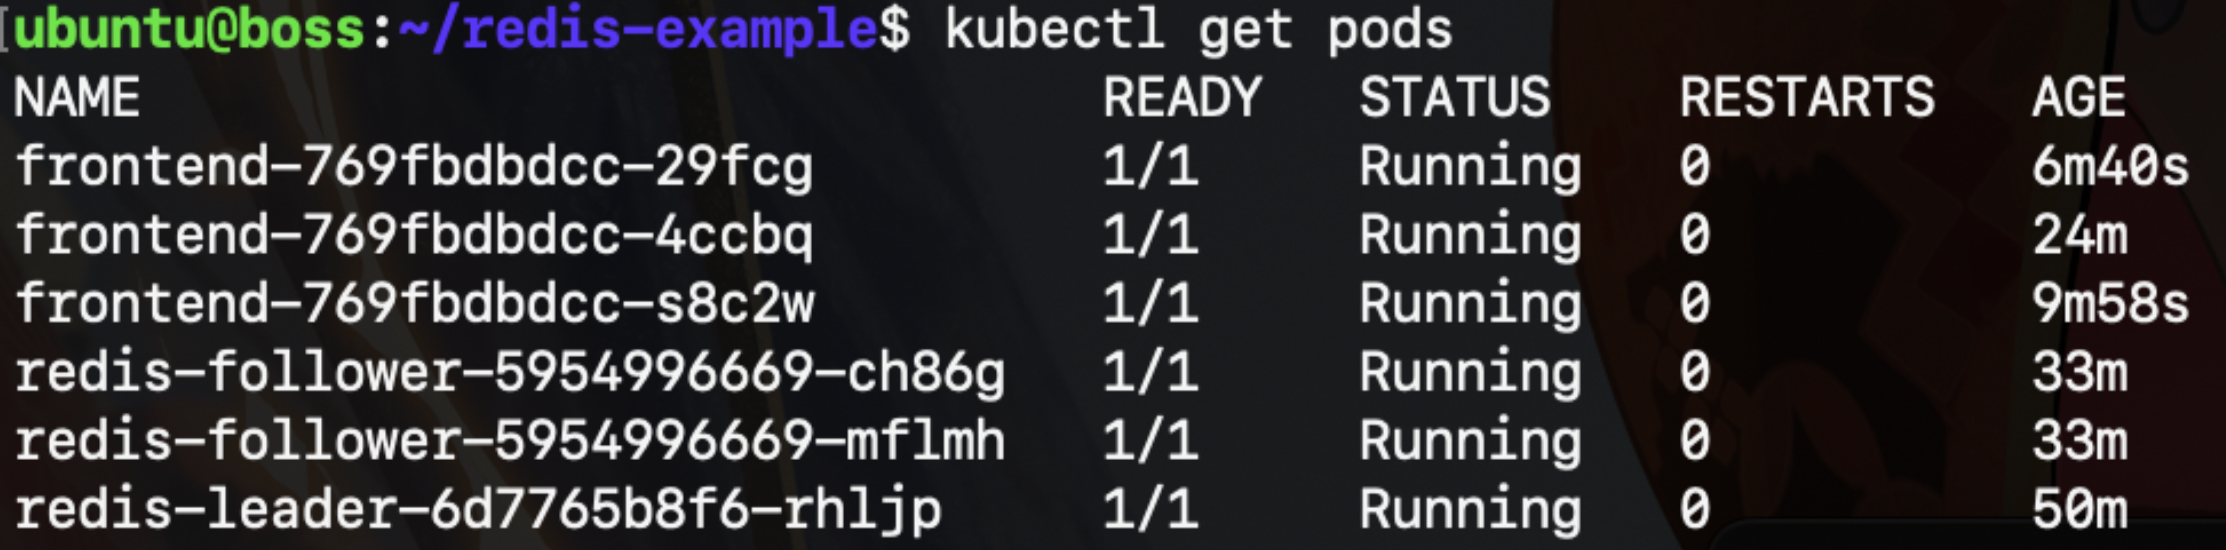
\includegraphics[width=\textwidth]{podsall.png}
        \caption{全部的实例信息}
        \label{fig:podsall}
    \end{subfigure}
    \hfill
    \begin{subfigure}[b]{0.50\textwidth}
        \centering
        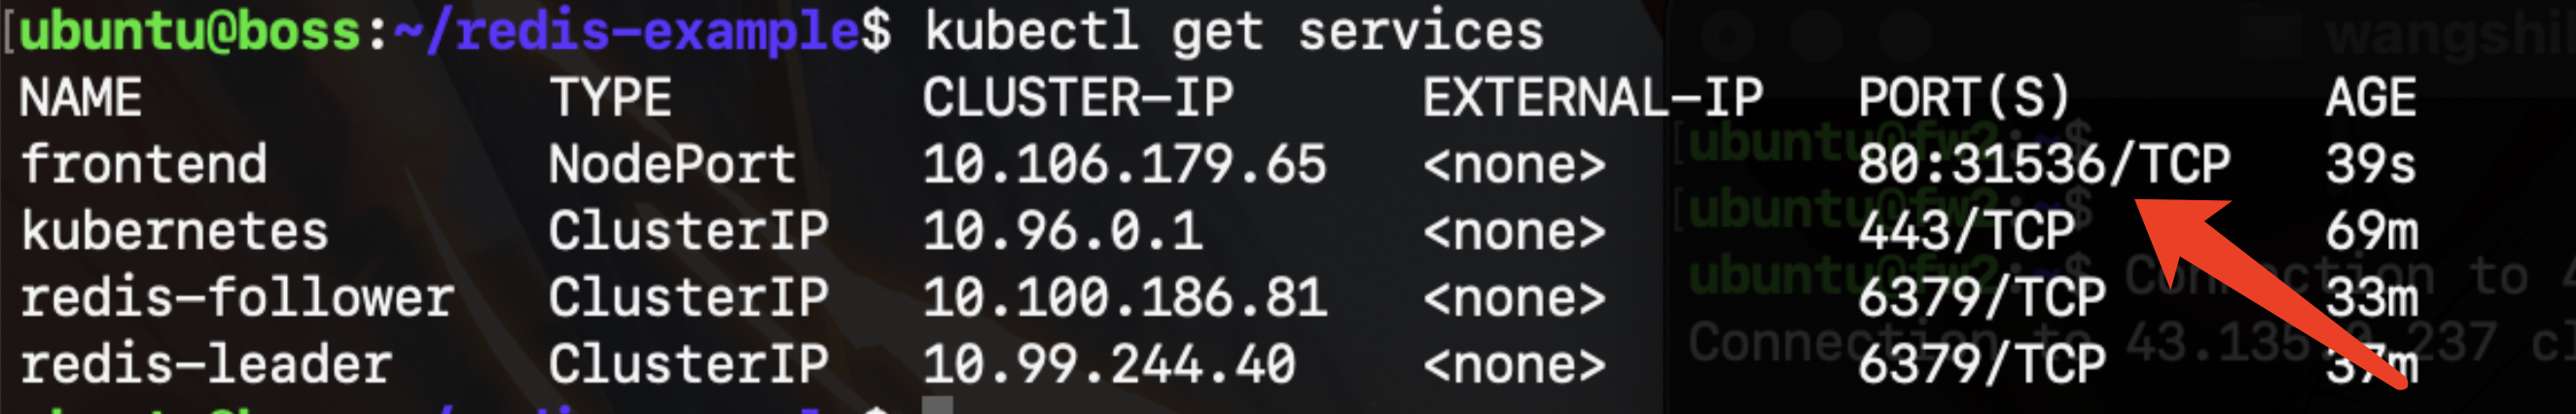
\includegraphics[width=\textwidth]{service1.png}
        \caption{获取所有的服务信息}
        \label{fig:service1}
    \end{subfigure}
\end{figure}

frontend部署了一个网页用于访问redis数据库,这个网页通过访问redis数据库来获取数据,然后
这个网站的读写会通过负载均衡分配给各个实例或者节点进行处理。
\begin{figure}[H]
    \centering
    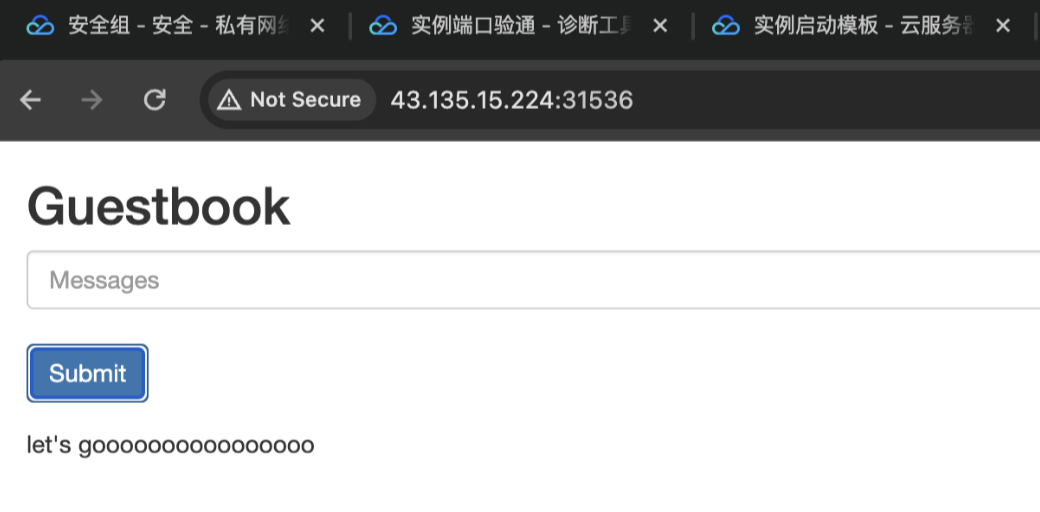
\includegraphics[width=0.6\textwidth]{webpage.png}
    \caption{网页访问}
    \label{fig:webpage}
\end{figure}

kubernetes提供了快速恢复的功能,对于异常终止的实例,kubernetes会自动重启实例,并且十分
快速,这样就保证了服务的持续可用性。并且kubernetes可以
通过\texttt{kubectl scale deployment \$\{NAME\} --replicas=\$\{NUM\}}
来进行扩容和缩容,这样就可以根据实际的需求来调整实例的数量,十分灵活和方便。
看下面的第一行是使用\texttt{kubectl delete frontend-769fbdbdcc-4ccbg}终止的实例,可以看到
快速恢复,因为和其他实例运行时间不一样。第二行是通过\texttt{kubectl scale deployment frontend --replicas=5}
增加的两个实例。
\begin{figure}[H]
    \begin{subfigure}[b]{0.45\textwidth}
        \centering
        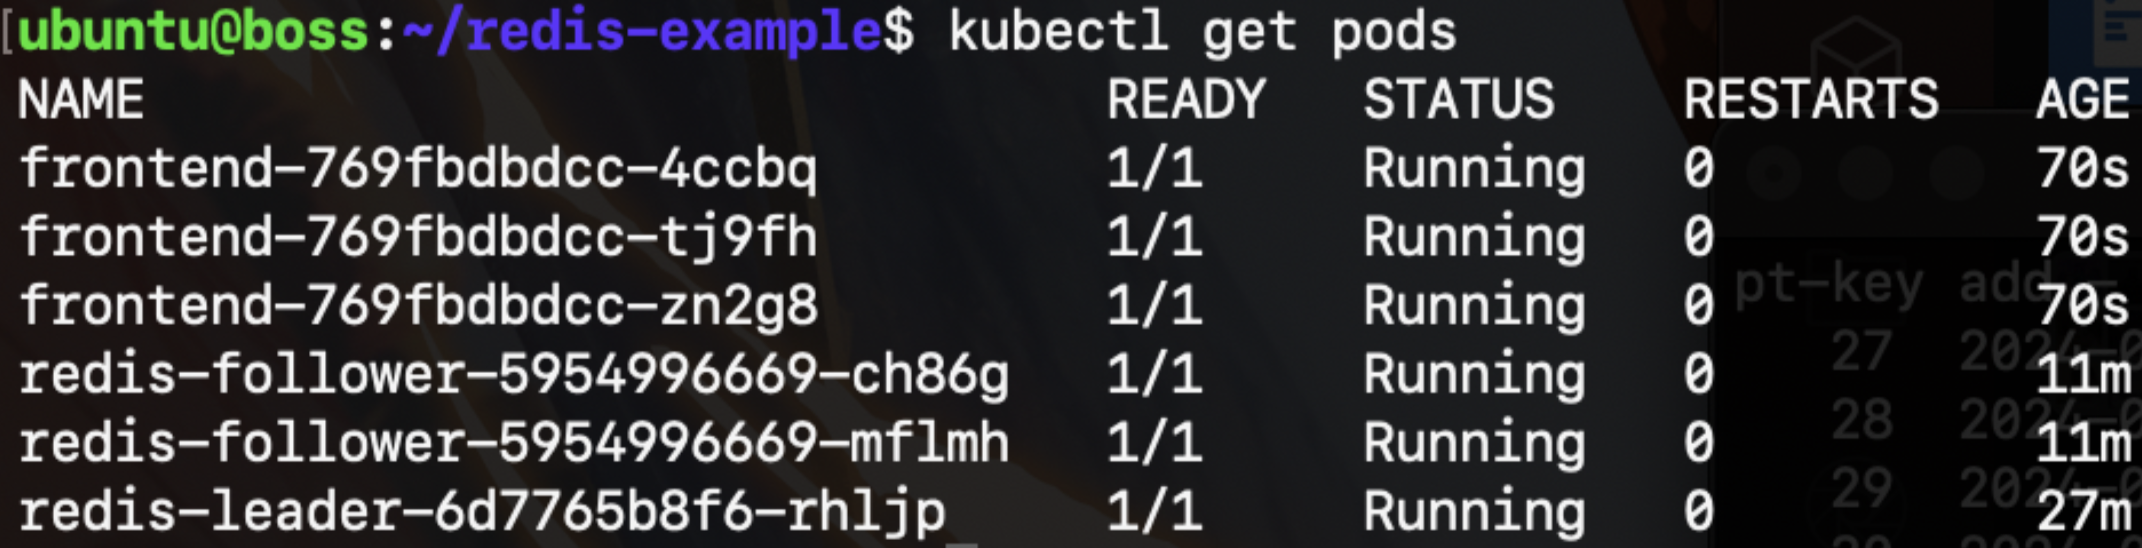
\includegraphics[width=\textwidth]{cos1.png}
        \caption{扩容和停止之前的实例信息}
        \label{fig:cos1}
    \end{subfigure}
    \hfill
    \begin{subfigure}[b]{0.50\textwidth}
        \centering
        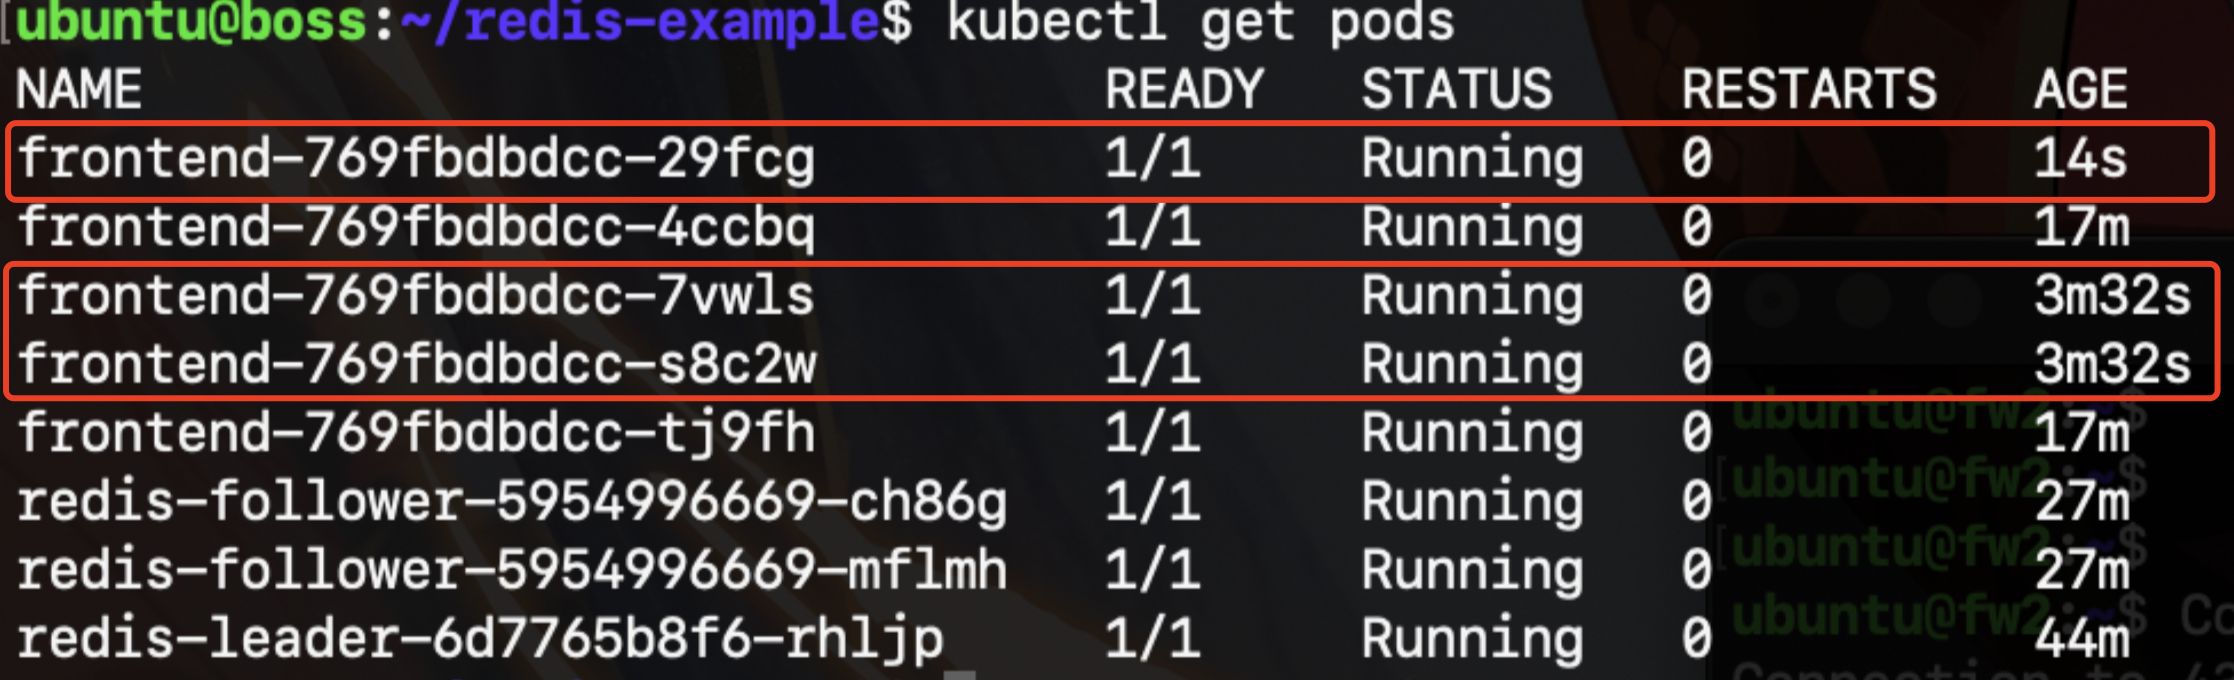
\includegraphics[width=\textwidth]{cos2.png}
        \caption{扩容和停止之后的实例信息}
        \label{fig:cos2}
    \end{subfigure}
\end{figure}
\section{实验感想}
\end{document}